\documentclass[sigconf]{acmart}
%%% Local Variables:
%%% ispell-local-dictionary: "english"
%%% End:
\usepackage[utf8]{inputenc}
\usepackage{booktabs} % For formal tables
\usepackage{graphicx}
\usepackage{rotating}
\definecolor{Gray}{gray}{0.6}

\setcopyright{rightsretained}

% DOI
\acmDOI{10.1145/nnnnnnn.nnnnnnn}

% ISBN
\acmISBN{978-x-xxxx-xxxx-x/YY/MM}


%Conference
\acmConference[GECCO '18]{the Genetic and Evolutionary Computation
Conference 2018}{July 15--19, 2018}{Kyoto, Japan}
\acmYear{2018}
\copyrightyear{2018}


\acmArticle{4}
\acmPrice{15.00}

\begin{document}

\title{Mapping evolutionary algorithms to a reactive, stateless architecture}
\subtitle{Using a modern concurrent language}


\author{Juan J. Merelo}
\orcid{1234-5678-9012}
\affiliation{%
  \institution{Universidad de Granada}
  \streetaddress{Daniel Saucedo Aranda, s/n}
  \city{Granada}
  \country{Spain}
}
\email{jmerelo@ugr.es}

\author{José-Mario García-Valdez}
\affiliation{%
  \institution{Instituto Tecnológico de Tijuana}
  \streetaddress{Calzada Tecnológico, s/n}
  \city{Tijuana}
  \country{Mexico}
}
\email{mario@tectijuana.edu.mx}

% The default list of authors is too long for headers.
\renewcommand{\shortauthors}{J. J. Merelo et al.}

\begin{abstract}
\keywords{concurrent programming, distributed evolutionary algorithms}
\end{abstract}

\begin{CCSXML}
<ccs2012>
<concept>
<concept_id>10003752.10003809.10003716.10011136.10011797.10011799</concept_id>
<concept_desc>Theory of computation~Evolutionary algorithms</concept_desc>
<concept_significance>500</concept_significance>
</concept>

<concept>
<concept_id>10010520.10010521.10010537.10003100</concept_id>
<concept_desc>Computer systems organization~Cloud computing</concept_desc>
<concept_significance>500</concept_significance>
</concept>

<concept>
<concept_id>10010147.10010919.10010172</concept_id>
<concept_desc>Computing methodologies~Distributed algorithms</concept_desc>
<concept_significance>300</concept_significance>
</concept>
</ccs2012>
\end{CCSXML}

\ccsdesc[500]{Theory of computation~Evolutionary algorithms}

\ccsdesc[300]{Computing methodologies~Distributed algorithms}

\keywords{Microservices, distributed computing,
  event-based systems, Kappa architecture, stateless algorithms,
  algorithm implementation, performance evaluation, distributed
  computing, pool-based systems, heterogeneous distributed systems,
  serverless computing, functions as a service.}

\maketitle

\section{Introduction}

\noindent Genetic algorithms (GA) \cite{GA_Goldberg89} are currently
one of the most widely used meta-heuristics to solve engineering
problems. Furthermore, parallel genetic algorithms (pGAs) are useful
to find  solutions of complex optimizations problems in adequate times
\cite{Luque2011}; in particular, problems with complex fitness. Some
authors \cite{Alba2001} state that using pGAs improves the quality of
solutions in terms of the number of evaluations needed to find
one. This reason, together with the improvement in evaluation time
brought by the simultaneous running in several nodes, have made
parallel and distributed evolutionary algorithms a popular
methodology. 

Implementing  evolutionary algorithms in parallel is relatively straightforward,
but programming paradigms used for the implementation of such
algorithms is far from being an object of study. Object oriented or
procedural languages like Java and C/C++ are mostly used. Even when
some researchers show that implementation matters
\cite{DBLP:conf/iwann/MereloRACML11}, parallels approaches in new
languages/paradigms is not normally seen as a land for scientific
improvements. 

New parallel platforms have been identified as new trends in pGAs \cite{Luque2011}, however only hardware is considered. Software platforms, specifically programming languages, remain poorly explored; only Ada \cite{Santos2002} and Erlang \cite{A.Bienz2011,Kerdprasop2013} were slightly tested.

The multicore’s challenge \cite{SutterL05} shows a current need for making parallel even the simplest program. But this way leads us to use and create design patterns for concurrent algorithms; the conversion of a pattern into a language feature is a common practice in the programming languages domain, and sometimes that means a language modification, others the creation of a new one. 

This work explores the advantages of Perl6
\cite{Tang:2007:PRI:1190216.1190218},  a relatively new and decidedly
non mainstream languages, since it is not included in the top ten of
any most popular languages ranking) with concurrent and functional
features in order to develop EAs in its parallel versions through
concurrency. This paper, as well as similar ones preceding it \cite{DBLP:conf/gecco/CruzGGC13,Albert-Cruz2014169}, is
motivated by the lack of community attention on the subject and the
belief that using concepts that simplify the modeling and
implementation of such algorithms might promote their use in research
and in practice. 

This research is intended to show some possible areas of improvement on architecture and engineering best practices for concurrent-functional paradigms, as was made for Object Oriented Programming languages \cite{EO:FEA2000}, by focusing on pGAs as a domain of application and describing how their principal traits can be modeled by means of concurrent-functional languages constructs. We are continuing the research reported in \cite{DBLP:conf/gecco/CruzGGC13,J.Albert-Cruz2013}.
%other papers (hidden for double-blind review).

The rest of the paper is organized as follows. Next section presents the state of the art in concurrent and functional programming language paradigms and its potential use for implementing pGAs. We present two different versions of a concurrent evolutionary algorithm in Section \ref{sec:impl}, to be followed by actual results in section \ref{sec:res}. Finally, we draw the conclusions and present future lines of work in section \ref{sec:conclusions}.

\section{State of the Art}

\noindent Developing correct software quickly and efficiently is a
never ending goal in the software industry. Novel solutions that try
to make a difference providing new abstraction tools outside the
mainstream of programming languages have been proposed to pursue this
goal; two of the most promising are the functional and the concurrent.

The concurrent programming paradigm (or concurrency oriented
programming \cite{Armstrong2003}) is characterized by the presence of
programming constructs for managing processes like first class
objects. That is, with operators for acting upon them and the
possibility of using them like parameters or function's result
values. This simplifies the coding of concurrent algorithms due to the
direct mapping between patterns of communications and processes with
language expressions. 

Concurrent programming is hard for many reasons, the communication/synchronization between processes is key in the design of such algorithms. One of the best efforts to formalize and simplify that is the Hoare’s {\em Communicating Sequential Processes} \cite{Hoare:1978:CSP:359576.359585}, this interaction description language is the theoretical support for many libraries and new programming languages.

When a concurrent programming language is used normally it has a
particular way of handling units of execution, being independent of
the operation system has several advantages: one program in those
languages will work the same way on different operating systems. Also
they can efficiently manage a lot of processes even on a
mono-processor machine.


Functional programming paradigm, despite its advantages, does not have
many followers. Several years ago was used in Genetic Programming
\cite{Briggs:2008:FGP:1375341.1375345,Huelsbergen:1996:TSE:1595536.1595579,walsh:1999:AFSFESIHLP}
and recently in neuroevolution \cite{Sher2013} but in GA its presence
is practically nonexistent \cite{Hawkins:2001:GFG:872017.872197}. 

This paradigm is characterized by the use of functions as first
class concepts, and for discouraging the use of state changes, with
functions mapping directly input to output without having any side effect. The
latter is particularly useful for develop concurrent algorithms in
which the communication by state changes is the origin of errors and
complexity. Also, functional features like closures and first class
functions in general, allow to express in one expression patterns like
\emph{observer} which in language like Java need so many lines and
files of source code.

The field of programming languages research is very active in the
Computer Science discipline. To find software construction tools with
new and better means of algorithms expression is welcome. In the last
few years the functional and concurrent paradigms have produced a rich
mix in which concepts of the first one had been simplified by the use
of the second ones. 

Among this new generation, the languages Erlang and Scala have
embraced the actor model of concurrency and get excelentes results in
many application domains; Clojure is another one with concurrent
features such as promises/futures, Software Transaction Memory and
agents. All of these tools have processes like built-in types and
scale beyond the restrictions of the number of OS-threads. On the
other hand, Perl 6 \cite{Tang:2007:PRI:1190215.1190218} uses different
concurrency models, that go from implicit concurrency using a
particular function that automatically parallelizes operations on
iterable data structures, to explicit concurrency using threads. These
both types of concurrency will be analyzed in this paper.

\section{Concurrent evolutionary algorithms and its implementation}
\label{sec:impl}

The implementation of evolutionary algorithms in a concurrent
environment must have several features:\begin{itemize}
\item They must be {\em reactive}, that is, functions respond to
  events, and not procedural or sequential.
\item Functions responding to events are also first class objects and
  are stateless, having no secondary effects. These functions have to
  be reentrant, that is, with the capability of being run in a thread
  without exclusion of other functions.
\item Functions communicate with each other exclusively via channels, which can
  hold objects of any kind but are not cached or buffered. Channels
  can be shared, but every object can be read from a channel only
  once.
\end{itemize}

In general, an evolutionary algorithm consists of an interative
procedure where, after generating an initial set of individuals, these
individuals are evaluated, and then they reproduce, with errors and
combination of their features, with a probability
that is proportional to their fitness. As long as there is variation
and survival of the fittest, an evolutionary algorithm will
work. However, the  usual way of doing this is through a series of
nested loops, with possibly asynchronous operation in a parallel
context when communicating with other {\em islands} or isolated
populations. However, the concept of loop itself implies state, in the
shape of the generation counter, or even with the population itself
that is handled from one iteration step to the next one.

Getting rid of these states, however, leads to many different
algorithms which are not functionally equivalent to the canonical
genetic algorithm above. Of course, a functional equivalent is also
possible in this environment, with non-terminating {\em islands}
running every one of them on a different thread, and communicating via
channels. Although this version is guaranteed to succeed, we are
looking for different implementations that, while keeping the spirit
of the evolutionary algorithm, maps themselves better to a
multithreaded architecture and a concurent language such as Go, Scala
or Perl 6.

This is why in this paper we are going to examine two different
architectures, which basically differ in the granularity with which
they perform the evolutionary algorithm.

\subsection{Individual-level concurrency}
\label{ss:indi}
%
\begin{figure*}[t!bp]
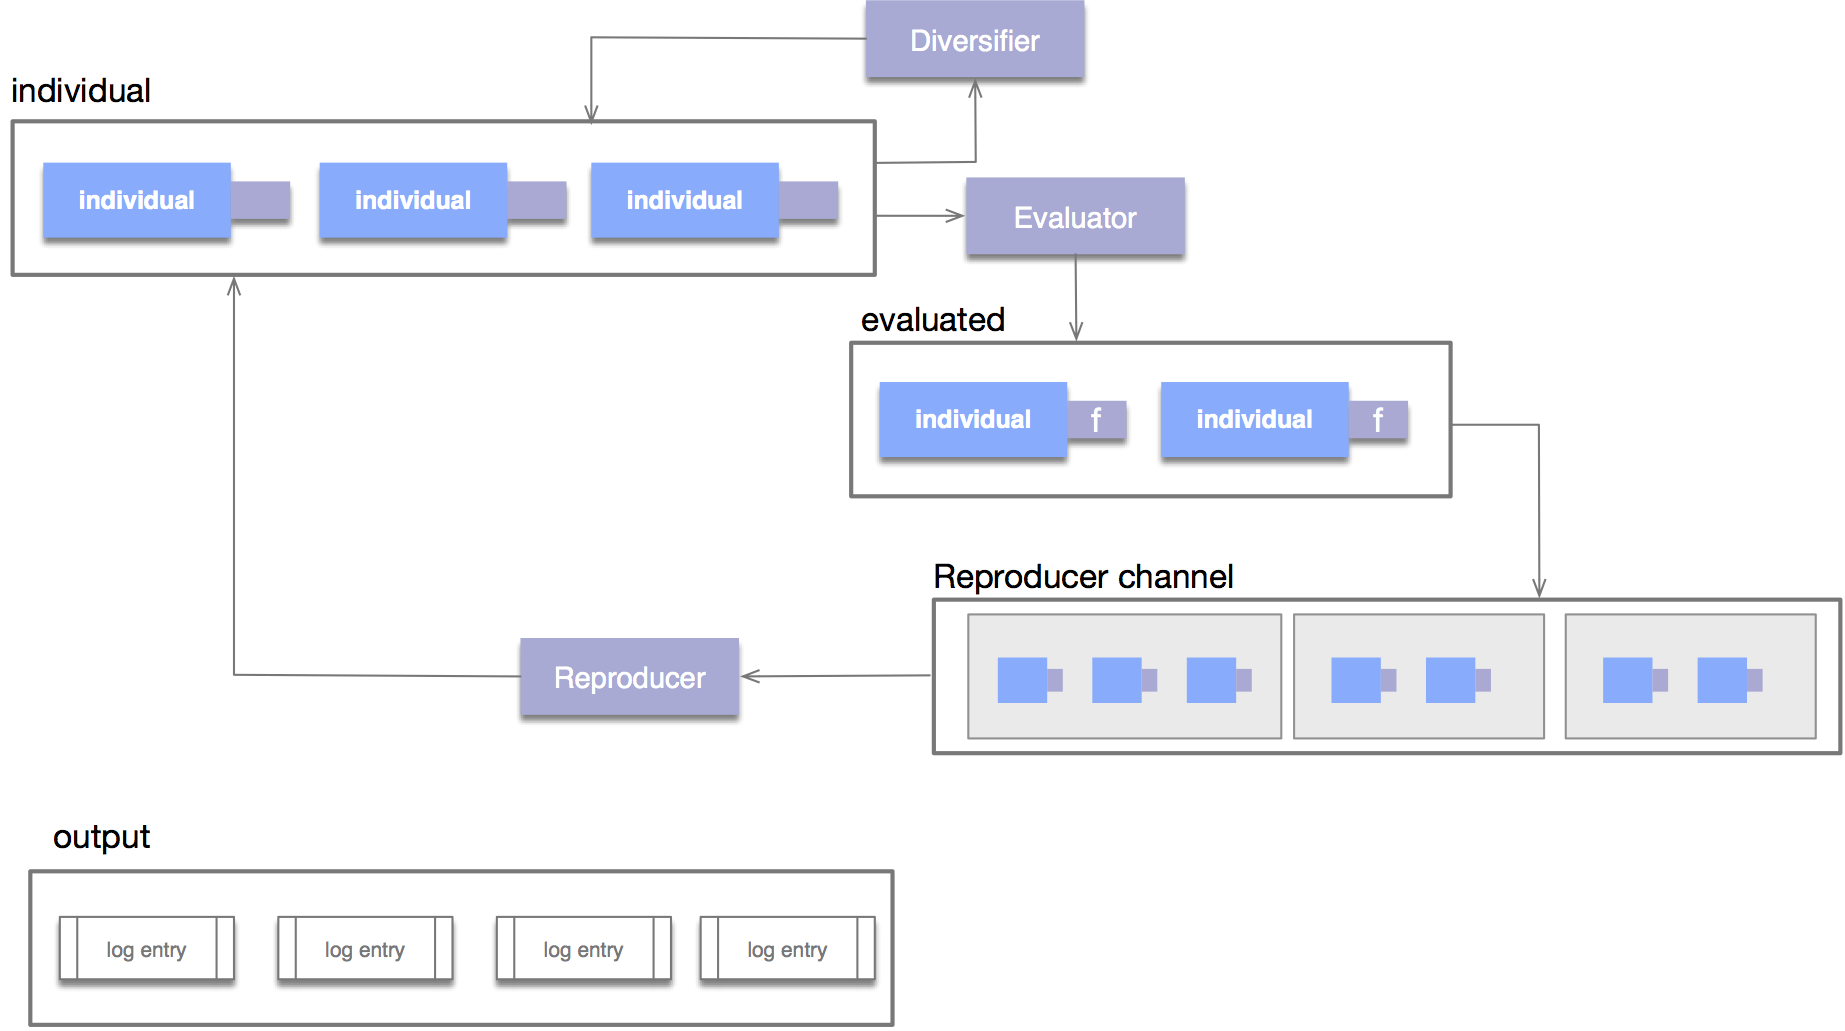
\includegraphics[width=0.95\textwidth]{channels-individual.png}
\caption{Channels and functions used in the individual-level concurrency version of the algorithm. }
\label{fig:indi}
\end{figure*}


In this version of the algorithm, all functions operate on single individuals or sets of them. We are going to use three different channels:\begin{itemize}
\item Channel {\sf individual}, which contains chromosomes without a fitness
  function. A subchannel of this channel takes the chromosomes in groups.
\item Channel {\sf evaluated}, which contains chromosomes paired with
  their fitness function. This channel receives individuals one by
  one, but emits them in groups of three.
\item Channel {\sf output}, which is used for logging what is
  happening in the other two channels and printing output at the end
  of the experiment.
\end{itemize}

There are two functions feeding these channels. \begin{itemize}
  
\item {\sf Evaluator} reacts to the {\sf individual} channel, picking and evaluating a single individual and emits it to the {\sf evaluated} as
  well as {\sf output} channel as an object that contains the original chromosome and the computed fitness. 
\item {\sf Reproducer} picks three individuals from the {\sf
    evaluated} channel, generates a new couple using crossover, and
  emits it to the {\sf individual} channel. This function also acts as
  selector, and in fact it is similar to 3 tournament, since it takes three individuals and returns only two of them to the channel, along with the two individuals that have been generated via crossover and mutation. 
\item {\sf Diversifier} is a re-broadcasting of the {\sf individual
    channel}, picks a group of individuals and shuffles it, putting it
  back into the same channel, giving them a different order in the
  buffer.
\end{itemize}

How channels and functions relate to and communicate with each other is represented in Figure \ref{fig:indi}.  The functions described above rebroadcast the values they read from the cannel when needed to other channels so that all
channels are kept fed and a deadlock situation is not produced. This
could happen, for instance, if the {\sf reproducer channel}, which
takes individuals in pairs, is only able to read a single one; since it is waiting for
a second individual it is not producing new ones and the algorithm
will stall. This could be fixed in a different way by changing from a reactive architecture to a {\em polling} architecture, but that kind of architecture also introduces overhead by polling when it is not needed. You have to balance when designing these types of algorithms, anyway; polling is another possibility, but one we are not exploring in this paper. 

The concurrency of this situation implies that we can run as many
copies as available of every one of them. Also that there is an
initial process where you generate the initial population, a series of
individuals which must be even, and bigger than the number of
individuals used in the diversifier. This is equivalent to an initial
population, although in this case there is no real {\em population},
since individuals are considered in groups of three. 

Depending on the overhead emission and reception adds, it is possible
that the performance of this channel is not the adequate one, even if
theoretically it is sound. That is why we have also proposed next a
coarse-grained version where the function process whole populations.

\subsection{Population-level concurrency}

In this case, the algorithm uses a single channel that emits and receives
populations. However, this channel is also re-broadcast as another channel
that takes the population in pairs. Having a single channel, even is with
different threads, will make several threads concurrently process
populations that will evolve in complete independence. This is why
there are two functions: \begin{itemize}
\item {\sf Singles} takes single populations and evolves them for a
  number of generations. It stops if it finds the solution, and closes
  the channel at the same time.
\item {\sf Pairs} reads pairs of populations from the sub-channel and
  mixes them, creating a new population with the best members of both
  populations. This {\em mixer} is equivalent to a process of
  migration that takes members from one population to another. Since
  this function takes two elements from the channel, it must leave two
  elements in the channel too. What it does is it emits back a
  randomly chosen population in the pair. 
\end{itemize}

Additionally, there must be a function, which can be concurrent, to
create the initial population. The process of migration performed by
the mixer is needed to overcome the {\em stateless}
nature of the concurrent process. The state is totally contained in
the population; the mixer respects this state of affairs by using only this information to perform the evolutionary algorithm.

\subsection{Notes on implementation using Perl 6}

Perl 6 \cite{Tang:2007:PRI:1190215.1190218} has been chosen to perform
the implementation of these two different versions of a concurrent
evolutionary algorithm. This choice has been due mainly to the
existence of an open source evolutionary algorithm library, recently
released by the authors and called {\tt
  Algorithm::Evolutionary::Simple}. This library, released to the
repository of common Perl 6 modules and called CPAN, includes
functions for the implementation of a very simple evolutionary
algorithm for optimizing onemax, Royal Road or any other benchmark
function.

Perl 6 \cite{lenzperl} is, despite its name, a language that is
completely different from Perl, designed for scratch to implement most
modern language features: meta-object protocols, concurrency, and
functional programming. It does not have a formal grammar, but is
rather defined by the tests a compiler or interpreter must pass in
order to be called ``Perl 6''. 
It consists of a virtual machine and a just in
time compiler which is written mostly in Perl 6 itself, so that it can
be easily ported from one virtual machine to others. Although it can
target many different virtual machines, the current ``official''
implementation includes a virtual machine called MoarVM and a compiler
called Rakudo. All together they compose the so-called {\em Rakudo
  start} distribution, a {\em stable} distribution of compiler +
virtual machine that is released every 4 monts from GitHub and to
package repositories. 

The advantage of using Perl 6 is that it combines the expressivity of
an interpreted language with the power of concurrency. Not very many
languages nowadays include concurrency as a base feature; Go, Scala
and Erlang are some of them. The concurrency in Go is done in a
similar way to Perl 6, using channels, but Go is a compiled,
non-functional language.

The main disadvantage of Perl 6 is raw performance, which is much
slower than Go, although in general, similar although slower than
other interpreted languages such as Python or Perl. Language
performance is not an static feature, and it usually improves with
time; in a separate paper, we have proved how speed has increased by
orders of magnitude since it was released a few years ago.

This paper, however, is focused on the algorithmic performance more
than the raw performance, so suffice it to say that Perl 6 performance
was adequate for running these experiments in a reasonable amount of
time.

The module used, as well as the code for the experiments, is available
under a free license. 

\section{Experimental setup and results}
\label{sec:res}

In order to perform the experiments, we used Linux boxes (with Ubuntu
14.04 and 16.04), the latest version of the Perl 6 compiler and
virtual machine. 


\section{Conclusions}
\label{sec:conclusions}

\begin{acks}

  This paper has been supported in part by
projects TIN2014-56494-C4-3-P s (Spanish Ministry of Economy and
Competitiveness) and DeepBio (TIN2017-85727-C4-2-P)


\end{acks}


\bibliographystyle{ACM-Reference-Format}
\bibliography{geneura,concurrent,perl6}

\end{document}
